\documentclass[11pt,a4paper]{ctexart}
\usepackage[teacher]{../../../common/ipara}
\usepackage{mathtools}
\usepackage{longtable}
\raggedbottom

\pagestyle{fancy}
\fancyhf{}
\lhead{\small 第三套卷子解析}
\cfoot{\small 第 \thepage\ 页}
\renewcommand{\headrulewidth}{0.4pt}

\newcommand{\R}{\mathbb{R}}
\newcommand{\ans}[1]{\(\boxed{#1}\)}

\begin{document}

\begin{center}
  {\zihao{2}\bfseries 第三套卷子详细解析}\\[2mm]
  \rule{0.86\linewidth}{0.5pt}
\end{center}

\section{单选题详细解析}

\subsection*{第 1 题：复数模长计算}
若 $z=-3+4i$，则 $|z|=$ (\quad) \\
A. 12 \qquad B. 1 \qquad C. $\sqrt5$ \qquad D. 5

\teachblock{考点}{
复数模的定义。
}

\begin{paracol}{2}
\teachblock{标准解答}{
根据复数模的定义，若 $z=a+bi$ ($a,b\in\mathbb{R}$)，则其模为：
$$|z|=\sqrt{a^2+b^2}$$
代入 $z=-3+4i$ 得：
$$|z|=\sqrt{(-3)^2+4^2}=\sqrt{9+16}=5$$
故选 \ans{D}。
}
\switchcolumn
\teachblock{教学建议与技巧}{
本题属于基础送分题。可以通过勾股数 $(3,4,5)$ 直接秒杀。
}
\end{paracol}

\subsection*{第 2 题：对数的运算}
若 $m\in \mathbb{R}$，$\lg 2^{51}=m+30.351$，$\lg 2\approx0.301$，则 $m=$ (\quad) \\
A. $-16$ \qquad B. $-15$ \qquad C. $-14$ \qquad D. $-13$

\teachblock{考点}{
对数的性质（幂的对数）。
}

\begin{paracol}{2}
\teachblock{标准解答}{
由对数的性质可知：
$$\lg 2^{51}=51\lg 2$$
已知 $\lg 2\approx0.301$，代入计算得：
$$\lg 2^{51}\approx 51\times0.301 = 15.351$$
所以：
$$m+30.351 = 15.351$$
解得：
$$m = 15.351 - 30.351 = -15$$
故选 \ans{B}。
}
\switchcolumn
\teachblock{教学建议与技巧}{
计算 $51\times0.301$ 时可以拆开算：$51\times0.3 + 51\times0.001 = 15.3 + 0.051 = 15.351$，这样不易算错。
}
\end{paracol}

\subsection*{第 3 题：充分必要条件判断}
若命题 $p:x>2$，命题 $q:x<3$，则 $p$ 是 $\neg q$ 的 (\quad) \\
A. 充分不必要条件 \qquad B. 必要不充分条件 \\
C. 充要条件 \qquad D. 既不充分也不必要条件

\teachblock{考点}{
充分条件与必要条件的判定、常用逻辑用语。
}

\begin{paracol}{2}
\teachblock{标准解答}{
首先写出命题 $q$ 的否定。
因为 $q:x<3$，所以：
$$\neg q:x\ge3$$
我们要判断 $p:x>2$ 与 $\neg q:x\ge3$ 之间的推出关系：
\begin{itemize}
  \item 若 $\neg q$ 成立，即 $x\ge3$，则必有 $x>2$ 成立，即：
  $$\neg q \Longrightarrow p$$
  这说明 $p$ 是 $\neg q$ 的必要条件；
  \item 若 $p$ 成立，即 $x>2$，不一定能推出 $x\ge3$（例如取 $x=2.5$ 满足 $p$ 但不满足 $\neg q$），即：
  $$p \not\Longrightarrow \neg q$$
  这说明 $p$ 不是 $\neg q$ 的充分条件；
\end{itemize}
综上所述，$p$ 是 $\neg q$ 的必要不充分条件。
故选 \ans{B}。
}
\switchcolumn
\teachblock{教学建议与技巧}{
“$p$ 是 $r$ 的必要条件”等价于 $r \Longrightarrow p$。学生在此处容易混淆推出方向，建议用集合包含关系记忆：小集合能推出大集合，大集合是小集合的必要条件。
}
\end{paracol}

\subsection*{第 4 题：正切函数的对称中心}
函数 $f(x)=3\tan\left(2x+\frac{\pi}{6}\right)$ 图像的对称中心坐标为 (\quad) \\
A. $\left(\frac{k\pi}{2}-\frac{\pi}{12},0\right)(k\in\mathbb{Z})$ \qquad
B. $\left(\frac{k\pi}{2}-\frac{\pi}{3},0\right)(k\in\mathbb{Z})$ \\
C. $\left(\frac{k\pi}{4}-\frac{\pi}{12},0\right)(k\in\mathbb{Z})$ \qquad
D. $\left(\frac{k\pi}{4}-\frac{\pi}{6},0\right)(k\in\mathbb{Z})$

\teachblock{考点}{
正切函数的图像与性质、对称中心。
}

\begin{paracol}{2}
\teachblock{标准解答}{
正切函数 $y=\tan x$ 的对称中心为 $\left(\frac{k\pi}{2}, 0\right)$ （$k\in\mathbb{Z}$）。
令 $2x+\frac{\pi}{6} = \frac{k\pi}{2}$，
解得 $2x = \frac{k\pi}{2} - \frac{\pi}{6}$，
$$x = \frac{k\pi}{4} - \frac{\pi}{12} \quad (k\in\mathbb{Z})$$
所以函数 $f(x)$ 图像的对称中心坐标为 $\left(\frac{k\pi}{4}-\frac{\pi}{12}, 0\right)$ （$k\in\mathbb{Z}$）。
故选 \ans{C}。
}
\switchcolumn
\teachblock{易错提醒}{
学生极易将正切函数的对称中心误记为 $(k\pi, 0)$，从而漏掉正切函数在渐近线处的中心对称性（虽然在渐近线处无定义，但图像在两侧无限趋近，依然构成中心对称）。因此必须强调正切函数对称中心的横坐标满足 $x = \frac{k\pi}{2}$。
}
\end{paracol}

\subsection*{第 5 题：正四面体中异面直线所成角}
如图，在棱长均为 2 的正四面体 $A-BCD$ 中，$E,F$ 分别为 $CD,BC$ 的中点，则 $AE,EF$ 所成角的余弦值为 (\quad) \\
A. $\frac{\sqrt3}{6}$ \qquad B. $\frac{\sqrt{33}}6$ \qquad C. $\frac13$ \qquad D. $-\frac{\sqrt2}{6}$

\begin{center}
\begin{tikzpicture}[scale=1.5, >=stealth]
  \coordinate (B) at (0,0);
  \coordinate (C) at (3,0);
  \coordinate (D) at (1.2,0.8);
  \coordinate (A) at (1.5,2.5);
  
  \coordinate (E) at ($(C)!0.5!(D)$);
  \coordinate (F) at ($(B)!0.5!(C)$);
  
  \draw[dashed, gray] (B) -- (D);
  \draw[dashed, gray] (A) -- (D);
  \draw[dashed, gray] (C) -- (D);
  
  \draw[thick] (A) -- (B) -- (C) -- cycle;
  \draw[thick] (A) -- (C);
  
  \draw[thick, blue] (A) -- (E);
  \draw[thick, blue] (E) -- (F);
  \draw[dashed, blue] (A) -- (F);
  
  \fill (A) circle (1.5pt) node[above] {$A$};
  \fill (B) circle (1.5pt) node[below left] {$B$};
  \fill (C) circle (1.5pt) node[below right] {$C$};
  \fill (D) circle (1.5pt) node[right] {$D$};
  \fill (E) circle (1.5pt) node[right] {$E$};
  \fill (F) circle (1.5pt) node[below] {$F$};
\end{tikzpicture}
\end{center}

\teachblock{考点}{
异面直线所成角、余弦定理、空间向量法。
}

\begin{paracol}{2}
\teachblock{标准解答（纯几何法）}{
连接 $AF$。
因为 $A-BCD$ 是棱长为 2 的正四面体，所以各个面都是边长为 2 的正三角形。
在正 $\triangle ACD$ 中，$E$ 是 $CD$ 的中点，所以 $AE$ 为高线，
$$AE = \sqrt{2^2 - 1^2} = \sqrt{3}$$
同理，在正 $\triangle ABC$ 中， $F$ 是 $BC$ 的中点，
$$AF = \sqrt{3}$$
在 $\triangle BCD$ 中，$E,F$ 分别是 $CD,BC$ 的中点，所以 $EF$ 是中位线，
$$EF = \frac{1}{2}BD = 1$$
在 $\triangle AEF$ 中，由余弦定理得：
$$\cos\angle AEF = \frac{AE^2 + EF^2 - AF^2}{2AE \cdot EF} = \frac{3+1-3}{2\sqrt{3}\cdot 1} = \frac{1}{2\sqrt{3}} = \frac{\sqrt{3}}{6}$$
因为 $\frac{\sqrt{3}}{6} > 0$，所以 $AE$ 与 $EF$ 所成角的余弦值为 $\frac{\sqrt{3}}{6}$。
故选 \ans{A}。
}
\switchcolumn
\teachblock{标准解答（向量法）}{
取 $\vec{CA}=\vec a, \vec{CB}=\vec b, \vec{CD}=\vec d$ 为基底，则其模长均为 2，且两两夹角为 $60^\circ$（数量积 $\vec a\cdot\vec b=\vec a\cdot\vec d=\vec b\cdot\vec d=2$）。
因为 $E,F$ 分别为 $CD,BC$ 的中点，所以：
$$\vec{CE} = \frac{1}{2}\vec d, \quad \vec{CF} = \frac{1}{2}\vec b$$
从而 $\vec{EA} = \vec a - \frac{1}{2}\vec d$，$\vec{EF} = \frac{1}{2}\vec b - \frac{1}{2}\vec d$。
计算其数量积：
$$\vec{EA}\cdot\vec{EF} = \left(\vec a - \frac{1}{2}\vec d\right)\cdot\left(\frac{1}{2}\vec b - \frac{1}{2}\vec d\right)$$
$$= \frac{1}{2}\vec a\cdot\vec b - \frac{1}{2}\vec a\cdot\vec d - \frac{1}{4}\vec d\cdot\vec b + \frac{1}{4}\vec d^2$$
$$= 1 - 1 - \frac{1}{2} + 1 = \frac{1}{2}$$
又 $|\vec{EA}| = \sqrt{3}, |\vec{EF}| = 1$。
所以：
$$\cos\langle\vec{EA}, \vec{EF}\rangle = \frac{\vec{EA}\cdot\vec{EF}}{|\vec{EA}||\vec{EF}|} = \frac{\frac{1}{2}}{\sqrt{3}\cdot 1} = \frac{\sqrt{3}}{6}$$
故选 \ans{A}。
}
\end{paracol}

\subsection*{第 6 题：函数图像的识别}
若函数 $f(x)$ 的图象如下图所示，则 $f(x)$ 的解析式可能为 (\quad) \\
A. $f(x)=\pi^{|x|}+\frac{\sin x}{x^2+1}+1$ \qquad
B. $f(x)=\pi^{-|x|}+\frac{\cos^2x}{x^2+1}$ \\
C. $f(x)=\pi^{-|x|}+\frac{\sin x}{x^2+1}+1$ \qquad
D. $f(x)=\pi^{-|x|}+\frac{\cos x}{x^2+1}$

\begin{center}
\begin{tikzpicture}[scale=1.2, >=stealth]
  % Axes
  \draw[->] (-4.2,0) -- (4.2,0) node[below] {$x$};
  \draw[->] (0,-0.8) -- (0,2.5) node[left] {$f(x)$};
  \node[below left] at (0,0) {$O$};
  
  % Ticks
  \foreach \x in {-3,-2,-1,1,2,3}
    \draw (\x,0.05) -- (\x,-0.05);
  \node[below] at (2,0) {$2$};
  \node[below] at (-2,0) {$-2$};
  
  \foreach \y in {0.5,1,1.5,2}
    \draw (0.05,\y) -- (-0.05,\y);
  \node[left] at (0,1) {$1$};
  \node[left] at (0,2) {$2$};
  
  % We plot B's formula directly with a high sampling rate to keep the cusp sharp at x=0
  % Note: we avoid pgfmath parser bugs on negative values by rewriting x^2 to x*x and cos(x)^2 to cos(x)*cos(x)
  \draw[thick, blue, domain=-3.8:3.8, samples=201] 
    plot (\x, {exp(-1.14473*abs(\x)) + (cos(deg(\x))*cos(deg(\x)))/(\x*\x + 1)});
\end{tikzpicture}
\end{center}

\teachblock{考点}{
函数图象识别、奇偶性、特殊值、函数值正负判定。
}

\begin{paracol}{2}
\teachblock{标准解答}{
首先分析图像的数学特征：
\begin{enumerate}
  \item 图像关于 $y$ 轴对称，说明 $f(x)$ 为偶函数；
  \item 图像始终在 $x$ 轴上方，即 $f(x) \ge 0$；
  \item 当 $x=0$ 时，$f(0)=2$。
\end{enumerate}

【排除 A、C】：\\
因为 $\sin(-x) = -\sin x$，所以 $\frac{\sin x}{x^2+1}$ 是奇函数。
故 A、C 两项的解析式均不具有奇偶性，不关于 $y$ 轴对称，由此排除 A、C。

排除 D：
对于 B、D 两项，均满足为偶函数且 $f(0)=2$。
我们代入特殊值 $x=\pi$。
对于 D 项，其函数值为：
$$f(\pi) = \pi^{-\pi} + \frac{\cos\pi}{\pi^2+1} = \pi^{-\pi} - \frac{1}{\pi^2+1}$$
因为 $\pi^{-\pi} \approx 0.027$，而 $\frac{1}{\pi^2+1} \approx 0.092$，所以：
$$f(\pi) < 0$$
这与图像始终在 $x$ 轴上方矛盾，故排除 D。

对于 B 项，其函数值为：
$$f(\pi) = \pi^{-\pi} + \frac{\cos^2\pi}{\pi^2+1} = \pi^{-\pi} + \frac{1}{\pi^2+1} > 0$$
符合图像始终在 $x$ 轴上方的特征。
故选 \ans{B}。
}
\switchcolumn
\teachblock{教学建议与技巧}{
图像选择题的核心在于“排除法”。通常的判定顺序为：
1. 奇偶性（对称性）；
2. 特殊值（如 $x=0$ 处的取值）；
3. 极限趋势（如 $x \to \infty$）；
4. 符号（是否会穿过 $x$ 轴）。
本题中代入 $x=\pi$ 排除 D 是非常经典的“特殊值定正负”的技巧。
}
\end{paracol}

\subsection*{第 7 题：分层抽样的总体方差}
已知某大厂的甲、乙车间生产的圆钢数之比为 $2:3$，现在要对甲、乙两个车间生产这种圆钢的直径进行误差抽检，具体要求为按比例分层抽检 50 根，若抽检的甲、乙车间圆钢的直径误差的平均值分别为 $1.1\text{ mm}, 1.05\text{ mm}$，误差的方差分别为 $0.5\text{ mm}^2, 0.45\text{ mm}^2$，则可以估计甲、乙车间的总体误差的方差约为 (\quad) \\
A. $0.686\text{ mm}^2$ \qquad B. $1.07\text{ mm}^2$ \qquad C. $0.4706\text{ mm}^2$ \qquad D. $0.475\text{ mm}^2$

\teachblock{考点}{
分层抽样的样本均值与方差。
}

\begin{paracol}{2}
\teachblock{标准解答}{
由题意可知，甲、乙两个车间占总体的比例（权重）分别为 $w_1 = \frac{2}{5} = 0.4$，$w_2 = \frac{3}{5} = 0.6$。
总体均值 $\bar{x} = w_1\bar{x}_1 + w_2\bar{x}_2$
$$= 0.4\times 1.1 + 0.6\times 1.05 = 0.44 + 0.63 = 1.07$$
根据分层抽样的方差公式，总体方差 $s^2$ 由“组内方差的加权平均”与“组间均值的偏差波动”两部分组成：
$$s^2 = \sum_{i=1}^2 w_i\left[s_i^2 + (\bar{x}_i - \bar{x})^2\right]$$
代入数据得：
$$s^2 = 0.4\times\left[0.5 + (1.1 - 1.07)^2\right] + 0.6\times\left[0.45 + (1.05 - 1.07)^2\right]$$
$$= 0.4\times(0.5 + 0.0009) + 0.6\times(0.45 + 0.0004)$$
$$= 0.4\times 0.5009 + 0.6\times 0.4504$$
$$= 0.20036 + 0.27024 = 0.4706\text{ mm}^2$$
故选 \ans{C}。
}
\switchcolumn
\teachblock{教学建议与技巧}{
【快速估算法】：
因为两车间的均值 $1.1$ 和 $1.05$ 非常接近，组间偏差 $(\bar{x}_i - \bar{x})^2$ 极小。
因此总体方差主要取决于组内方差的加权平均：
$$s^2 \approx 0.4\times 0.5 + 0.6\times 0.45 = 0.2 + 0.27 = 0.47\text{ mm}^2$$
真实总体方差应当比 $0.47$ 略大一点点。观察选项，C项 $0.4706$ 完美符合，可以直接锁定。
}
\end{paracol}

\subsection*{第 8 题：球与大圆面的翻折垂直问题}
如图，已知球 $O$ 的半径为 1，两个大圆面 $PAQ,PBQ$ 互相垂直，$\angle AOQ=\angle BOQ=\frac{2\pi}{3}$，若平面 $AOB$ 与平面 $PBQ$ 的夹角为 $\alpha$，则 (\quad) \\
A. $AB=\frac{\sqrt6}{2},\tan\alpha=2$ \qquad
B. $AB=\frac{\sqrt6}{2},\tan\alpha=\frac{2\sqrt5}{5}$ \\
C. $AB=\frac{\sqrt3}{2},\tan\alpha=2$ \qquad
D. $AB=1,\tan\alpha=\frac12$

\begin{center}
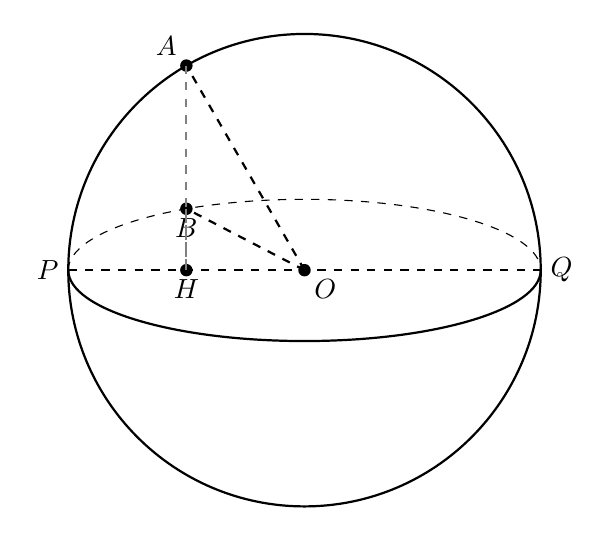
\begin{tikzpicture}[scale=1.5, >=stealth]
  % Outer sphere boundary
  \draw[thick] (0,0) circle (2);
  
  % Horizontal axis PQ
  \draw[dashed, thick] (-2,0) -- (2,0);
  \node[left] at (-2,0) {$P$};
  \node[right] at (2,0) {$Q$};
  \node[below right] at (0,0) {$O$};
  \fill (0,0) circle (1.5pt);
  
  % Horizontal ellipse (great circle)
  \draw[thick] (2,0) arc [start angle=0, end angle=-180, x radius=2, y radius=0.6];
  \draw[dashed] (-2,0) arc [start angle=180, end angle=0, x radius=2, y radius=0.6];
  
  % Coordinates
  \coordinate (A) at (-1, 1.732);
  \coordinate (B) at (-1, 0.52); % 0.6 * sin(120) = 0.6 * 0.866 = 0.5196
  \coordinate (H) at (-1, 0);
  
  % Connect OA, OB, AB
  \draw[dashed, thick] (0,0) -- (A);
  \draw[dashed, thick] (0,0) -- (B);
  \draw[dashed, thick] (A) -- (B);
  
  % Labels
  \fill (A) circle (1.5pt) node[above left] {$A$};
  \fill (B) circle (1.5pt) node[below] {$B$};
  
  % Helper point H and lines
  \fill (H) circle (1.5pt) node[below] {$H$};
  \draw[dashed, gray, thick] (A) -- (H);
  \draw[dashed, gray, thick] (B) -- (H);
\end{tikzpicture}
\end{center}

\teachblock{考点}{
面面垂直的性质、二面角的几何求法、空间距离计算。
}

\begin{paracol}{2}
\teachblock{标准解答}{
【第一步：利用面面垂直作投影】
因为大圆面必过球心 $O$，所以两圆面的交线为球的直径 $PQ$，且 $P,O,Q$ 三点共线。
由平面 $PAQ \perp$ 平面 $PBQ$，在平面 $PAQ$ 内，过点 $A$ 向交线 $PQ$ 作垂线，垂足为 $H$。
由面面垂直 of 性质定理可知，$AH \perp$ 平面 $PBQ$。
在平面 $PAQ$ 中，因为 $OA=1$，且 $\angle AOQ = 120^\circ$，
所以 $H$ 落在 $OQ$ 的反向延长线（即射线 $OP$）上，且：
$$OH = |OA\cos 120^\circ| = \frac{1}{2}$$
$$AH = OA\sin 120^\circ = \frac{\sqrt{3}}{2}$$

【第二步：求线段 $AB$ 的长度】
在平面 $PBQ$ 中，因为 $\angle BOQ = 120^\circ$，而 $H$ 在 $OQ$ 的反向延长线上，所以 $\angle BOH = 60^\circ$。
在 $\triangle BOH$ 中，由余弦定理得：
$$BH^2 = OB^2 + OH^2 - 2OB\cdot OH\cos 60^\circ$$
$$= 1^2 + \left(\frac{1}{2}\right)^2 - 2\times 1\times\frac{1}{2}\times\frac{1}{2} = \frac{3}{4} \quad\Longrightarrow\quad BH = \frac{\sqrt{3}}{2}$$
因为 $AH \perp$ 平面 $PBQ$，且 $BH \subset$ 平面 $PBQ$，所以 $AH \perp BH$。
在直角 $\triangle ABH$ 中，由勾股定理得：
$$AB = \sqrt{AH^2 + BH^2} = \sqrt{\frac{3}{4} + \frac{3}{4}} = \frac{\sqrt{6}}{2}$$

【第三步：求二面角正切值 $\tan\alpha$】
平面 $AOB$ 与平面 $PBQ$ 的交线为 $OB$。
在平面 $PBQ$ 中，过 $H$ 向交线 $OB$ 作垂线，垂足为 $K$，即 $HK \perp OB$。
因为 $AH \perp$ 平面 $PBQ$，由三垂线定理逆定理可知，$AK \perp OB$。
所以 $\angle AKH$ 即为平面 $AOB$ 与平面 $PBQ$ 的夹角 $\alpha$。
在 $\triangle BOH$ 中，因为 $OH = \frac{1}{2}$，$\angle BOH = 60^\circ$，
所以点 $H$ 到直线 $OB$ 的距离 $HK = OH\sin 60^\circ = \frac{1}{2}\times\frac{\sqrt{3}}{2} = \frac{\sqrt{3}}{4}$。
in 直角 $\triangle AKH$ 中：
$$\tan\alpha = \frac{AH}{HK} = \frac{\frac{\sqrt{3}}{2}}{\frac{\sqrt{3}}{4}} = 2$$
综上所述，$AB = \frac{\sqrt{6}}{2}$，$\tan\alpha = 2$。
故选 \ans{A}。
}
\switchcolumn
\teachblock{教学建议与几何直观}{
本立体几何题难度较大，极其考验学生的空间想象能力和几何降维能力。
1. \textbf{建立局部直角关系}：利用“面面垂直 $\rightarrow$ 线面垂直”确定 $AH \perp$ 平面 $PBQ$，是破题关键。
2. \textbf{利用二面角定义找平面角}：找交线 $OB$，然后利用三垂线定理在 $\triangle BOH$ 中做高线 $HK$，从而确定平面角 $\alpha$ 的位置。整个过程避免了复杂的建系和法向量计算，纯几何法极其高效。
}
\end{paracol}

\newpage

\section{多选题详细解析}

\subsection*{第 9 题：统计量概念比较}
在某次高三模拟考试后，数学老师统计了第一组的 8 名同学第 19 题的得分情况如下：$(7,9,5,8,5,3,3,3)$，第二组的 8 名同学第 19 题的得分情况如下：$(8,10,6,9,6,4,4,4)$，则 (\quad) \\
A. 第二组的平均数比较大 \qquad B. 两组的中位数之差的绝对值为 1 \\
C. 两组的众数相等 \qquad D. 两组的极差相等

\teachblock{考点}{
平均数、中位数、众数、极差的计算与性质。
}

\begin{paracol}{2}
\teachblock{标准解答}{
观察数据特征，发现第二组的每一个得分均比第一组的对应得分大 1，
即 $X_{\text{II}} = X_{\text{I}} + 1$。
根据统计量在线性变换下的变化性质：
\begin{itemize}
  \item 平均数满足 $\bar{X}_{\text{II}} = \bar{X}_{\text{I}} + 1$，故第二组平均数大，A 正确；
  \item 中位数满足 $M_{\text{II}} = M_{\text{I}} + 1$，故两组中位数差的绝对值为 1，B 正确；
  \item 众数满足 $Mod_{\text{II}} = Mod_{\text{I}} + 1$，第一组众数为 3，第二组众数为 4，不相等，C 错误；
  \item 极差满足 $R_{\text{II}} = R_{\text{I}}$（因为最大值与最小值同时加上 1，差值保持不变），D 正确。
\end{itemize}
故选 \ans{ABD}。
}
\switchcolumn
\teachblock{数据验算}{
第一组排序：$3,3,3,5,5,7,8,9$。
中位数为 $\frac{5+5}{2}=5$，众数为 3，极差为 $9-3=6$。
第二组排序：$4,4,4,6,6,8,9,10$。
中位数为 $\frac{6+6}{2}=6$，众数为 4，极差为 $10-4=6$。
各项数据与整体变换规律完全一致。
}
\end{paracol}

\subsection*{第 10 题：旋转体的体积与表面积比}
若将 4 张铁皮进行任意无重叠地切割，分别可以焊接成底面半径均为 1、高均为 2 的一个密闭圆锥和一个密闭圆柱、上下底面半径分别为 $(\frac12,\frac32)$、高为 2 的一个密闭圆台及直径为 2 的一个球，不考虑损耗，则体积与其表面积之比最大的是 (\quad) \\
A. 球 \qquad B. 圆锥 \qquad C. 圆柱 \qquad D. 圆台

\teachblock{考点}{
球、圆柱、圆锥、圆台的体积与表面积计算公式。
}

\begin{paracol}{2}
\teachblock{标准解答}{
本题本质是比较各密闭几何体的 $\frac{V}{S}$ 的大小：
\begin{itemize}
  \item \textbf{A. 球}：直径为 2，则半径 $r=1$。\\
  体积为：
  $$V_{\text{球}} = \frac{4}{3}\pi r^3 = \frac{4}{3}\pi$$
  表面积为：
  $$S_{\text{球}} = 4\pi r^2 = 4\pi$$
  所以：
  $$\frac{V}{S} = \frac{\frac{4}{3}\pi}{4\pi} = \frac{1}{3}$$
  
  \item \textbf{B. 圆锥}：底面半径 $r=1$，高 $h=2$。\\
  母线长为：
  $$l = \sqrt{r^2+h^2} = \sqrt{5}$$
  体积为：
  $$V_{\text{锥}} = \frac{1}{3}\pi r^2 h = \frac{2}{3}\pi$$
  表面积为：
  $$S_{\text{锥}} = \pi r^2 + \pi r l = \pi(1+\sqrt{5})$$
  所以：
  $$\frac{V}{S} = \frac{2}{3(1+\sqrt{5})} \approx 0.21 < \frac{1}{3}$$
  
  \item \textbf{C. 圆柱}：底面半径 $r=1$，高 $h=2$。\\
  体积为：
  $$V_{\text{柱}} = \pi r^2 h = 2\pi$$
  表面积为：
  $$S_{\text{柱}} = 2\pi r^2 + 2\pi rh = 6\pi$$
  所以：
  $$\frac{V}{S} = \frac{2\pi}{6\pi} = \frac{1}{3}$$
  
  \item \textbf{D. 圆台}：上底半径 $r=\frac{1}{2}$，下底半径 $R=\frac{3}{2}$，高 $h=2$。\\
  母线长为：
  $$l = \sqrt{h^2+(R-r)^2} = \sqrt{5}$$
  体积为：
  $$V_{\text{台}} = \frac{1}{3}\pi h(R^2+Rr+r^2) = \frac{13}{6}\pi$$
  表面积为：
  $$S_{\text{台}} = \pi r^2 + \pi R^2 + \pi(R+r)l = \pi\left(\frac{5}{2}+2\sqrt{5}\right)$$
  所以：
  $$\frac{V}{S} = \frac{13}{15+12\sqrt{5}}$$
  比较 $\frac{13}{15+12\sqrt{5}}$ 与 $\frac{1}{3}$：因为 $39 < 15+12\sqrt{5}$，所以该比值小于 $\frac{1}{3}$。
\end{itemize}
综上所述，体积与表面积比最大的是球和圆柱。
故选 \ans{AC}。
}
\switchcolumn
\teachblock{教学建议与分析}{
密闭旋转体在体积固定时，越接近球体，其表面积利用率越高。
圆锥和圆台由于“收缩”使得侧面积分配不够饱满，$\frac{V}{S}$ 会变小。
球和高与直径相等的圆柱（即等边圆柱）恰好都达到了最大比值 $\frac{1}{3}$，这让很多学生感到意外，是个非常好的几何探究素材。
}
\end{paracol}

\subsection*{第 11 题：解三角形综合命题}
在 $\triangle ABC$ 中，三个角 $A,B,C$ 所对的边分别为 $a,b,c$，其外接圆的半径为 $R$，若 $b^2=ac$，则 (\quad) \\
A. $\triangle ABC$ 的面积为 $\frac{b^3}{4R}$ \qquad
B. $B\le \frac{\pi}{3}$ \\
C. $a+c<2b$ \qquad
D. $\frac{-1+\sqrt5}{2}<\frac ba<\frac{1+\sqrt5}{2}$

\teachblock{考点}{
三角形面积公式、正弦与余弦定理、基本不等式、三角形存在性条件。
}

\begin{paracol}{2}
\teachblock{标准解答}{
【对于 A】：\\
三角形面积公式为：
$$S = \frac{abc}{4R}$$
由已知 $b^2=ac$，代入得：
$$S = \frac{b\cdot ac}{4R} = \frac{b^3}{4R}$$
故 A 正确；

【对于 B】：\\
由余弦定理得：
$$\cos B = \frac{a^2+c^2-b^2}{2ac}$$
将 $b^2=ac$ 代入得：
$$\cos B = \frac{a^2+c^2-ac}{2ac}$$
由基本不等式 $a^2+c^2 \ge 2ac$，所以：
$$\cos B \ge \frac{2ac-ac}{2ac} = \frac{1}{2}$$
因为 $B\in(0,\pi)$，所以：
$$B \le \frac{\pi}{3}$$
故 B 正确；

【对于 C】：\\
由基本不等式可得：
$$a+c \ge 2\sqrt{ac} = 2b$$
所以 $a+c < 2b$ 恒不成立，故 C 错误；

【对于 D】：\\
设 $x = \frac{b}{a} > 0 \Rightarrow b = xa$。
由 $b^2=ac$ 得：
$$c = \frac{b^2}{a} = x^2 a$$
所以三边之比为：
$$a:b:c = 1:x:x^2$$
根据三角形三边关系：
\begin{enumerate}
  \item $a+b > c \Rightarrow 1+x > x^2 \Rightarrow x^2-x-1 < 0$，解得 $0 < x < \frac{1+\sqrt{5}}{2}$；
  \item $b+c > a \Rightarrow x+x^2 > 1 \Rightarrow x^2+x-1 > 0$，解得 $x > \frac{-1+\sqrt{5}}{2}$；
  \item $a+c > b \Rightarrow 1+x^2 > x \Rightarrow x^2-x+1 > 0$ 恒成立。
\end{enumerate}
联立解得：
$$\frac{-1+\sqrt{5}}{2} < \frac{b}{a} < \frac{1+\sqrt{5}}{2}$$
故 D 正确。

综上所述，正确的选项为 \ans{ABD}。
}
\switchcolumn
\teachblock{教学建议与技巧}{
1. \textbf{秒杀选项 C}：由等比数列性质，几何平均数 $\sqrt{ac} = b \le \frac{a+c}{2}$ 恒成立，因此 C 直接与基本不等式违背。
2. \textbf{三边关系的整体换元}：利用 $a:b:c = 1:x:x^2$ 的特征，将三角形存在性转化为一元二次不等式，这是解决此类等比三边问题（如黄金分割三角形）的通用套路，应进行专题总结。
}
\end{paracol}

\newpage

\section{填空题详细解析}

\subsection*{第 12 题：随机取数与差的绝对值}
从 $\{1,2,3,5\}$ 这四个数中随机取出 2 个不同的数，则它们差的绝对值为质数的概率为 \ans{\frac{1}{2}}。

\teachblock{考点}{
古典概型、质数的概念、分类讨论思想。
}

\begin{paracol}{2}
\teachblock{标准解答}{
从 4 个数中取 2 个不同的数，基本事件总数为：
$$C_4^2 = 6\text{ 种}$$

【解法一：列举所有无序取法】\\
分别列出所有可能的无序数对及其差的绝对值：
\begin{enumerate}
  \item $(1,2)$：$|1-2|=1$，1 不是质数；
  \item $(1,3)$：$|1-3|=2$，2 是质数；
  \item $(1,5)$：$|1-5|=4$，4 不是质数；
  \item $(2,3)$：$|2-3|=1$，1 不是质数；
  \item $(2,5)$：$|2-5|=3$，3 是质数；
  \item $(3,5)$：$|3-5|=2$，2 是质数。
\end{enumerate}
其中差的绝对值为质数的数对有：$(1,3)$, $(2,5)$, $(3,5)$，共 3 种。
所以所求概率为：
$$P = \frac{3}{6} = \frac{1}{2}$$

【解法二：按“差值”分类】\\
四个数可能产生的正差值有 $1, 2, 3, 4$。其中质数差值为 $2, 3$。
\begin{itemize}
  \item 差为 2 的数对有：$(1,3)$, $(3,5)$，共 2 对；
  \item 差为 3 的数对有：$(2,5)$，共 1 对。
\end{itemize}
所以有利情况共 $2+1=3$ 种。
所以所求概率为：
$$P = \frac{3}{6} = \frac{1}{2}$$
}
\switchcolumn
\teachblock{应试技巧与易错点}{
本题最容易错在\textbf{将 1 误判为质数}。
质数是大于 1 的自然数，且除了 1 和它本身外没有其他正因数。
因为 1 不是质数，所以差为 1 的数对 $(1,2)$ 和 $(2,3)$ 应当排除。
在考试中，快速筛选出差值为 2 或 3 的数对即可。
}
\end{paracol}

\subsection*{第 13 题：集合的交集运算}
若 $A=\{x \mid x=2k, k\in\mathbb{Z}\}$，$B=\{x \mid x=4k+1\text{ 或 }x=4k-1, k\in\mathbb{Z}\}$，则 $A\cap B = $ \ans{\varnothing}。

\teachblock{考点}{
集合的交集、奇数与偶数的概念、模运算与反证法。
}

\begin{paracol}{2}
\teachblock{标准解答}{
【解法一：看奇偶性】\\
集合 $A = \{x \mid x=2k, k\in\mathbb{Z}\}$ 表示所有偶数，即：
$$\{\dots, -4, -2, 0, 2, 4, \dots\}$$
集合 $B$ 中的元素满足 $x=4k+1$（必为奇数）或 $x=4k-1$（必为奇数）。
所以集合 $B$ 表示所有形如 $4k \pm 1$ 的奇数。
因为偶数集合与奇数集合没有公共元素，所以：
$$A\cap B = \varnothing$$

【解法二：用模运算理解】\\
集合 $A$ 中的元素满足：
$$x \equiv 0 \pmod 2$$
即所有偶数。
集合 $B$ 中的元素满足：
$$x \equiv 1 \pmod 4 \quad \text{或} \quad x \equiv -1 \equiv 3 \pmod 4$$
这正好是所有的奇数（因为奇数模 4 的余数只能是 1 或 3）。
所以集合 $A$ 表示偶数，集合 $B$ 表示奇数，二者无交集，即：
$$A\cap B = \varnothing$$

【解法三：反证法】\\
假设存在元素 $x \in A\cap B$。
因为 $x \in A$，所以 $x = 2k$ ($k\in\mathbb{Z}$)，即 $x$ 为偶数。
又因为 $x \in B$，所以 $x = 4t+1$ 或 $x = 4t-1$ ($t\in\mathbb{Z}$)，无论是哪一种，$x$ 均为奇数。
一个整数不可能既是奇数又是偶数，这与假设矛盾。
所以：
$$A\cap B = \varnothing$$
}
\switchcolumn
\teachblock{应试技巧}{
在高考中，这类集合交集题往往具有强烈的数论特征：
\begin{itemize}
  \item 看到 $2k$，立刻翻译为“偶数”；
  \item 看到 $4k \pm 1$，立刻翻译为“奇数”（因为偶数加减 1 必为奇数）。
\end{itemize}
无需进行任何代数化简或解方程，直接判定：
$$\text{偶数集合} \cap \text{奇数集合} = \varnothing$$
}
\end{paracol}

\subsection*{第 14 题：超越方程与代数式求值}
若方程 $e^{2x-1} = \frac{1-\ln x}{2x^2}$ 在 $(0,+\infty)$ 上有唯一解 $t$，则 $\frac{2t+\ln t}{2}$ 的值为 \ans{\frac{1}{2}}。

\teachblock{考点}{
超越方程的求解、构造函数、单调性分析、代数式整体换元。
}

\begin{paracol}{2}
\teachblock{标准解答}{
【解法一：构造目标式（特值/直觉法）】\\
题目要求求值的是 $\frac{2t+\ln t}{2}$，其核心在于确定 $2t+\ln t$ 的值。
原方程为：
$$e^{2x-1} = \frac{1-\ln x}{2x^2}$$
尝试令 $2x+\ln x = 1$，则：
$$\ln x = 1 - 2x$$
此时，方程右边化简为：
$$\frac{1-\ln x}{2x^2} = \frac{1 - (1-2x)}{2x^2} = \frac{2x}{2x^2} = \frac{1}{x}$$
而方程左边化简为：
$$e^{2x-1} = e^{-\ln x} = \frac{1}{e^{\ln x}} = \frac{1}{x}$$
此时左右两边相等。
这说明满足 $2x+\ln x = 1$ 的数一定是原方程的解。
因为方程在 $(0,+\infty)$ 上有唯一解 $t$，所以该解必满足：
$$2t+\ln t = 1$$
所以：
$$\frac{2t+\ln t}{2} = \frac{1}{2}$$

【解法二：严格代数推出】\\
从原方程出发：
$$e^{2x-1} = \frac{1-\ln x}{2x^2}$$
设 $y = 2x+\ln x - 1$，则 $2x-1 = y-\ln x$。
代入左边得：
$$e^{2x-1} = e^{y-\ln x} = \frac{e^y}{x}$$
又由 $y = 2x+\ln x - 1$ 可得 $\ln x = y+1-2x$，
代入右边的分子得：
$$1 - \ln x = 1 - (y+1-2x) = 2x-y$$
此时原方程化为：
$$\frac{e^y}{x} = \frac{2x-y}{2x^2}$$
两边乘以 $2x^2$（因为 $x>0$）得：
$$2xe^y = 2x-y \quad\Longrightarrow\quad y = 2x(1-e^y)$$
下面分析 $y$ 的符号：
\begin{itemize}
  \item 若 $y > 0$，则 $e^y > 1 \implies 1-e^y < 0$。因为 $x > 0$，所以右边 $2x(1-e^y) < 0$，与左边 $y > 0$ 矛盾；
  \item 若 $y < 0$，则 $e^y < 1 \implies 1-e^y > 0$。右边 $2x(1-e^y) > 0$，与左边 $y < 0$ 矛盾。
\end{itemize}
综上，只能有 $y = 0$，即：
$$2x+\ln x - 1 = 0$$
故原方程的唯一解 $t$ 满足 $2t+\ln t = 1$。
所以：
$$\frac{2t+\ln t}{2} = \frac{1}{2}$$

【解法三：辅助方程唯一解的严格论证】\\
设辅助函数 $g(x) = 2x+\ln x$。
在 $(0,+\infty)$ 上，$y=2x$ 严格递增，$y=\ln x$ 也严格递增，所以 $g(x)$ 严格递增。
又因为：
$$\lim_{x\to 0^+} g(x) = -\infty, \quad \lim_{x\to +\infty} g(x) = +\infty$$
所以方程 $2x+\ln x = 1$ 在 $(0,+\infty)$ 上有唯一实数解，设为 $x_0$。
根据解法一，该解 $x_0$ 满足原方程：
$$e^{2x_0-1} = \frac{1-\ln x_0}{2x_0^2}$$
而题目已知原方程在 $(0,+\infty)$ 上有且仅有唯一解 $t$，
所以必有 $t = x_0$。
故 $2t+\ln t = 1$，所以：
$$\frac{2t+\ln t}{2} = \frac{1}{2}$$
}
\switchcolumn
\teachblock{应试技巧}{
这道题是超越方程求值的经典题型。
\begin{itemize}
  \item \textbf{避开直接求解}：不要试图硬解出 $t$。因为方程 $e^{2x-1} = \frac{1-\ln x}{2x^2}$ 属于指、对、幂混合的超越方程，根本无法用初等函数求出具体根的数值。
  \item \textbf{整体代换特征}：注意题目所求的式子为 $\frac{2t+\ln t}{2}$，其中的核心部分 $2t+\ln t$ 与原方程中的指数位置 $2x-1$ 和对数位置 $\ln x$ 具有高度的结构关联，这强烈暗示我们需要寻找关于 $2t+\ln t$ 的整体等式，而不是单独求出 $t$。
\end{itemize}
}
\end{paracol}

\newpage

\section{解答题详细解析}

\subsection*{第 15 题：向量的垂直与平行}
已知 $\vec{a}=(1, \sin\theta), \vec{b}=(\cos\theta, t), \theta, t \in \mathbf{R}$.\\
(1) 若 $t=-1, \vec{a}\perp\vec{b}$，求 $\theta$；\\
(2) 若 $t=-\frac{\sqrt{3}}{4}, \vec{a}\parallel\vec{b}$，求 $\theta$.

\teachblock{考点}{
平面向量数量积、向量平行的坐标表示、三角函数化简。
}

\begin{paracol}{2}
\teachblock{标准解答}{
（1）因为 $t=-1$，所以 $\vec{b}=(\cos\theta, -1)$。
因为 $\vec{a}\perp\vec{b}$，所以 $\vec{a}\cdot\vec{b} = 0$，即
\[
1\cdot\cos\theta + \sin\theta\cdot(-1) = 0 \quad\Longrightarrow\quad \cos\theta = \sin\theta.
\]
于是 $\tan\theta = 1$。
解得 $\theta = \frac{\pi}{4} + k\pi, k \in \mathbf{Z}$。

（2）因为 $t=-\frac{\sqrt{3}}{4}$，所以 $\vec{b}=\left(\cos\theta, -\frac{\sqrt{3}}{4}\right)$。
因为 $\vec{a}\parallel\vec{b}$，所以
\[
1\cdot\left(-\frac{\sqrt{3}}{4}\right) - \sin\theta\cdot\cos\theta = 0.
\]
即 $\sin\theta\cos\theta = -\frac{\sqrt{3}}{4}$。
由二倍角公式得 $\frac{1}{2}\sin 2\theta = -\frac{\sqrt{3}}{4}$，即
\[
\sin 2\theta = -\frac{\sqrt{3}}{2}.
\]
解得 $2\theta = -\frac{\pi}{3} + 2k\pi$ 或 $2\theta = -\frac{2\pi}{3} + 2k\pi$ （$k \in \mathbf{Z}$）。
所以 $\theta = -\frac{\pi}{6} + k\pi$ 或 $\theta = -\frac{\pi}{3} + k\pi, k \in \mathbf{Z}$。
}

\switchcolumn
\teachblock{教学建议}{
本题属于基础的向量代数运算。
第一问容易漏掉周期 $k\pi$。
第二问的关键在于利用二倍角公式 $\sin 2\theta = 2\sin\theta\cos\theta$ 进行降次化简。
需要提醒学生最后写全解集。
}
\end{paracol}

\newpage

\subsection*{第 16 题：直三棱柱中的平行与垂直}
在直三棱柱 $ABC-A_1B_1C_1$ 中，已知 $D$ 为 $AC$ 的中点，$AB_1 \cap A_1B = O$.\\
(1) 求证：$OD \parallel \text{平面 } BCC_1B_1$；\\
(2) 若 $AB=BB_1=\sqrt{10}, BC=\sqrt{2}, AC=2\sqrt{3}$，证明：$A_1B \perp \text{平面 } AB_1C_1$.

\begin{center}
\begin{tikzpicture}[scale=1.2, >=stealth]
  \coordinate (A1) at (0,0);
  \coordinate (B1) at (4,0);
  \coordinate (C1) at (2.5,-1.5);
  
  \coordinate (A) at (0,3);
  \coordinate (B) at (4,3);
  \coordinate (C) at (2.5,1.5);
  
  \coordinate (D) at ($(A)!0.5!(C)$);
  \coordinate (O) at ($(A)!0.5!(B1)$); 
  
  % Dashed lines (back face and internal)
  \draw[dashed, thick] (A1) -- (B1);
  \draw[dashed, thick] (A) -- (B1);
  \draw[dashed, thick] (A1) -- (B);
  \draw[dashed, thick] (O) -- (D);
  \draw[dashed, thick] (A) -- (C1); % For plane AB1C1
  
  % Solid lines
  \draw[thick] (A) -- (B) -- (C) -- cycle;
  \draw[thick] (A1) -- (C1) -- (B1);
  \draw[thick] (A) -- (A1);
  \draw[thick] (B) -- (B1);
  \draw[thick] (C) -- (C1);
  
  \fill (A) circle (1pt) node[above left] {\(A\)};
  \fill (B) circle (1pt) node[above right] {\(B\)};
  \fill (C) circle (1pt) node[above right] {\(C\)};
  \fill (A1) circle (1pt) node[below left] {\(A_1\)};
  \fill (B1) circle (1pt) node[below right] {\(B_1\)};
  \fill (C1) circle (1pt) node[below] {\(C_1\)};
  \fill (D) circle (1pt) node[above right] {\(D\)};
  \fill (O) circle (1pt) node[right] {\(O\)};
\end{tikzpicture}
\end{center}

\begin{paracol}{2}
\teachblock{标准解答}{
（1）因为在直三棱柱中，四边形 $ABB_1A_1$ 为矩形，且 $AB_1 \cap A_1B = O$，
所以 $O$ 为 $AB_1$ 的中点。
又因为 $D$ 为 $AC$ 的中点，所以在 $\triangle AB_1C$ 中，$OD$ 是中位线。
故 $OD \parallel B_1C$。
又因为 $B_1C \subset \text{平面 } BCC_1B_1$，$OD \not\subset \text{平面 } BCC_1B_1$，
所以 $OD \parallel \text{平面 } BCC_1B_1$。

（2）因为 $AB=BB_1=\sqrt{10}$，所以矩形 $ABB_1A_1$ 是正方形，
因此其对角线互相垂直，即：
$$A_1B \perp AB_1$$
在底面 $\triangle ABC$ 中，$AB=\sqrt{10}, BC=\sqrt{2}, AC=2\sqrt{3}=\sqrt{12}$。
因为：
$$AB^2 + BC^2 = 10+2 = 12 = AC^2$$
满足勾股定理，故 $\angle ABC = 90^\circ$，即：
$$BC \perp AB$$
又因为三棱柱为直三棱柱，所以侧棱 $BB_1 \perp \text{底面 } ABC$，从而：
$$BB_1 \perp BC$$
因为 $AB \cap BB_1 = B$，所以：
$$BC \perp \text{平面 } ABB_1A_1$$
由棱柱的性质知 $B_1C_1 \parallel BC$，所以：
$$B_1C_1 \perp \text{平面 } ABB_1A_1$$
因为 $A_1B \subset \text{平面 } ABB_1A_1$，所以：
$$B_1C_1 \perp A_1B$$
又因为 $A_1B \perp AB_1$，$AB_1 \cap B_1C_1 = B_1$，且 $AB_1, B_1C_1 \subset \text{平面 } AB_1C_1$，
所以：
$$A_1B \perp \text{平面 } AB_1C_1$$
}

\switchcolumn
\teachblock{教学建议}{
（1）证明线面平行，核心是“找平行线”。在此题中，看到两个中点 $D$ 和 $O$，应立即想到中位线定理，在三角形 $AB_1C$ 中构造 $OD \parallel B_1C$。
（2）证明线面垂直，核心是“证线线垂直”。$A_1B$ 已经垂直于正方形的另一条对角线 $AB_1$，只需再找平面 $AB_1C_1$ 中的一条直线与其垂直。由于底面边长构成勾股数，顺理成章推导出 $BC \perp AB$，进而利用直棱柱性质证得 $BC$（即 $B_1C_1$）垂直于整个侧面 $ABB_1A_1$。这是非常经典的“面面垂直推线面垂直”的模型。
}
\end{paracol}

\newpage

\subsection*{第 17 题：三角恒等变换}
已知 $\alpha - \frac{\beta}{2}, \frac{\alpha}{2} - \beta$ 均为第一象限的角，且 $\sin\left(\alpha - \frac{\beta}{2}\right) = \frac{3}{5}, \cos\left(\frac{\alpha}{2} - \beta\right) = \frac{7}{25}$，求：\\
(1) $\sin\frac{3(\alpha - \beta)}{2}$ 的值；\\
(2) $\cos(\alpha + \beta)$ 的值.

\teachblock{考点}{
三角函数的和差化积、倍角公式、角变换技巧。
}

\begin{paracol}{2}
\teachblock{标准解答}{
设 $x = \alpha - \frac{\beta}{2}, y = \frac{\alpha}{2} - \beta$。
已知 $x, y$ 均为第一象限角，且 $\sin x = \frac{3}{5}, \cos y = \frac{7}{25}$。
所以 $\cos x = \sqrt{1 - \left(\frac{3}{5}\right)^2} = \frac{4}{5}$，$\sin y = \sqrt{1 - \left(\frac{7}{25}\right)^2} = \frac{24}{25}$。

（1）注意到 $x + y = \left(\alpha - \frac{\beta}{2}\right) + \left(\frac{\alpha}{2} - \beta\right) = \frac{3(\alpha - \beta)}{2}$。
所以 $\sin\frac{3(\alpha - \beta)}{2} = \sin(x+y) = \sin x \cos y + \cos x \sin y$
\[
= \frac{3}{5} \times \frac{7}{25} + \frac{4}{5} \times \frac{24}{25} = \frac{21}{125} + \frac{96}{125} = \frac{117}{125}.
\]

（2）注意到 $x - y = \left(\alpha - \frac{\beta}{2}\right) - \left(\frac{\alpha}{2} - \beta\right) = \frac{\alpha + \beta}{2}$。
则 $\cos\frac{\alpha + \beta}{2} = \cos(x-y) = \cos x \cos y + \sin x \sin y$
\[
= \frac{4}{5} \times \frac{7}{25} + \frac{3}{5} \times \frac{24}{25} = \frac{28}{125} + \frac{72}{125} = \frac{100}{125} = \frac{4}{5}.
\]
所以 $\cos(\alpha + \beta) = \cos\left(2 \cdot \frac{\alpha + \beta}{2}\right) = 2\cos^2\frac{\alpha + \beta}{2} - 1$
\[
= 2 \times \left(\frac{4}{5}\right)^2 - 1 = \frac{32}{25} - 1 = \frac{7}{25}.
\]
}
\switchcolumn
\teachblock{教学建议}{
（1）本题是经典的“整体换元”求值问题。必须让学生形成肌肉记忆：看到两个组合角，先尝试求它们的“和”与“差”。
（2）强调第一象限角的隐含条件，求另外的三角函数值时符号取正。
}
\end{paracol}

\newpage
\subsection*{第 18 题：解三角形综合}
如图，在平面四边形 $ABCD$ 中，已知 $AC, BD$ 交于 $O$, $AO = OC = \sqrt{2}, BD=2$, $\angle AOB = \frac{\pi}{4}$，且 $DO > BO$, 令 $\angle CDO = \alpha, \angle BAO = \beta$.\\
(1) 判断：$AB=CD$ 是否成立？请说明理由；\\
(2) 求 $\cos(\alpha - \beta)$ 的值；\\
(3) 证明：当 $\beta = \frac{\pi}{6}$ 时，$D$ 位于 $\triangle ABC$ 外接圆的内部.

\begin{center}
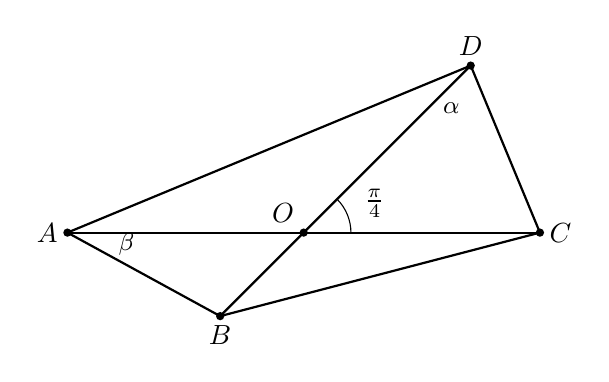
\begin{tikzpicture}[scale=1.5, >=stealth]
  \coordinate (O) at (0,0);
  \coordinate (A) at (-2, 0);
  \coordinate (C) at (2, 0);
  \coordinate (D) at (1.414, 1.414); 
  \coordinate (B) at (-0.707, -0.707); 
  
  \draw[thick] (A) -- (B) -- (C) -- (D) -- cycle;
  \draw[thick] (A) -- (C);
  \draw[thick] (B) -- (D);
  
  \fill (O) circle (1pt) node[above left] {$O$};
  \fill (A) circle (1pt) node[left] {$A$};
  \fill (B) circle (1pt) node[below] {$B$};
  \fill (C) circle (1pt) node[right] {$C$};
  \fill (D) circle (1pt) node[above] {$D$};
  
  \draw (0.4,0) arc (0:45:0.4);
  \node at (0.6, 0.25) {$\frac{\pi}{4}$};
  \node at (-1.5, -0.1) {\small $\beta$};
  \node at (1.25, 1.05) {\small $\alpha$};
\end{tikzpicture}
\end{center}

\begin{paracol}{2}
\teachblock{标准解答}{
（1）成立。理由如下：\\
设 $OB=x, OD=y$，则 $x+y=BD=2$。
在 $\triangle AOB$ 中，由余弦定理得：
$$AB^2 = OA^2 + OB^2 - 2OA \cdot OB \cos\frac{\pi}{4}$$
$$= 2 + x^2 - 2\sqrt{2}x \cdot \frac{\sqrt{2}}{2} = x^2 - 2x + 2$$
在 $\triangle COD$ 中，因为 $\angle COD = \angle AOB = \frac{\pi}{4}$，由余弦定理得：
$$CD^2 = OC^2 + OD^2 - 2OC \cdot OD \cos\frac{\pi}{4}$$
$$= 2 + y^2 - 2\sqrt{2}y \cdot \frac{\sqrt{2}}{2} = y^2 - 2y + 2$$
由于 $x+y=2$，即 $x = 2-y$，代入 $AB^2$ 得：
$$AB^2 = (2-y)^2 - 2(2-y) + 2$$
$$= 4 - 4y + y^2 - 4 + 2y + 2 = y^2 - 2y + 2 = CD^2$$
故 $AB = CD$ 恒成立。

（2）在 $\triangle COD$ 中，由余弦定理得：
$$\cos\alpha = \frac{OD^2 + CD^2 - OC^2}{2OD \cdot CD}$$
$$= \frac{y^2 + (y^2-2y+2) - 2}{2y \cdot CD} = \frac{2y(y-1)}{2y \cdot CD} = \frac{y-1}{CD}$$
在 $\triangle AOB$ 中，由余弦定理得：
$$\cos\beta = \frac{OA^2 + AB^2 - OB^2}{2OA \cdot AB}$$
$$= \frac{2 + (x^2-2x+2) - x^2}{2\sqrt{2} \cdot AB} = \frac{4-2x}{2\sqrt{2} \cdot AB} = \frac{2-x}{\sqrt{2}AB} = \frac{y}{\sqrt{2}AB}$$
同时，由正弦定理得：
$$\frac{OB}{\sin\beta} = \frac{AB}{\sin\frac{\pi}{4}} \quad\Longrightarrow\quad \sin\beta = \frac{x}{\sqrt{2}AB}$$
$$\frac{OC}{\sin\alpha} = \frac{CD}{\sin\frac{\pi}{4}} \quad\Longrightarrow\quad \sin\alpha = \frac{1}{CD} = \frac{1}{AB}$$
因为 $AB=CD$，所以：
$$\cos(\alpha - \beta) = \cos\alpha\cos\beta + \sin\alpha\sin\beta$$
$$= \frac{y-1}{AB} \cdot \frac{y}{\sqrt{2}AB} + \frac{1}{AB} \cdot \frac{x}{\sqrt{2}AB}$$
$$= \frac{y^2-y+x}{\sqrt{2}AB^2} = \frac{y^2-2y+2}{\sqrt{2}AB^2}$$
又 $AB^2 = y^2-2y+2$，故：
$$\cos(\alpha - \beta) = \frac{AB^2}{\sqrt{2}AB^2} = \frac{\sqrt{2}}{2}$$

（3）当 $\beta = \frac{\pi}{6}$ 时，$\cos\beta = \frac{\sqrt{3}}{2}$，即：
$$\frac{y}{\sqrt{2(y^2-2y+2)}} = \frac{\sqrt{3}}{2}$$
平方整理得：
$$4y^2 = 6(y^2-2y+2) \quad\Longrightarrow\quad y^2 - 6y + 6 = 0$$
解得 $y = 3 \pm \sqrt{3}$。
因为 $DO > BO \implies y > x \implies y > 1$，且 $y < BD = 2$，
所以 $y = 3 - \sqrt{3}$，此时 $x = 2-y = \sqrt{3}-1$。
在 $\triangle ABC$ 中，因为 $AC^2 = 8$，而：
$$AB^2 = x^2-2x+2 = (\sqrt{3}-1)^2 - 2(\sqrt{3}-1) + 2 = 8 - 4\sqrt{3}$$
$$BC^2 = OB^2 + OC^2 - 2OB \cdot OC \cos\frac{3\pi}{4}$$
$$= x^2 + 2 + 2x = (\sqrt{3}-1)^2 + 2 + 2(\sqrt{3}-1) = 4$$
所以：
$$AB^2 + BC^2 = 12 - 4\sqrt{3} < 8 = AC^2 \quad\Longrightarrow\quad \angle ABC > \frac{\pi}{2}$$
同理在 $\triangle ADC$ 中：
$$AD^2 = OA^2 + OD^2 - 2OA \cdot OD \cos\frac{3\pi}{4}$$
$$= 2 + y^2 + 2y = 2 + (3-\sqrt{3})^2 + 2(3-\sqrt{3}) = 20 - 8\sqrt{3}$$
$$CD^2 = y^2-2y+2 = 8-4\sqrt{3}$$
所以：
$$AD^2 + CD^2 = 28 - 12\sqrt{3} = 28 - \sqrt{432} < 8 = AC^2 \quad\Longrightarrow\quad \angle ADC > \frac{\pi}{2}$$
因为四边形 $ABCD$ 为凸四边形（对角线交于 $O$），且对角 $\angle ABC + \angle ADC > \pi$。
由圆内接四边形对角互补的性质可知，当对角和大于 $\pi$ 时，点 $D$ 必在 $\triangle ABC$ 外接圆的内部。
}
\switchcolumn
\teachblock{教学建议}{
（1）本题通过设 $OB=x, OD=y$，利用 $x+y=2$ 把两个三角形的余弦定理联系起来，证明 $AB=CD$ 是极其漂亮的代数消元法，完美避开了建系计算。
（2）第（3）问是典型的“判断点与圆的位置关系”。高中阶段最直接的判断标准是：对角互补关系。此处利用纯几何法计算出 $\angle B$ 和 $\angle D$ 均为钝角，从而 $\angle B + \angle D > \pi$，直接得出 $D$ 在 $\triangle ABC$ 外接圆内。纯几何代数推导干脆利落。
}
\end{paracol}

\newpage

\subsection*{第 19 题：概率综合与独立性检验}
在不透明的甲袋中装有相同的 6 个红色的乒乓球，其中 $a$ 个球上标有数字 1，$b$ 个球上标有数字 2，$6-a-b$ 个球上标有数字 3；在不透明的乙袋中装有相同的 3 个白色的乒乓球，其中 $m$ 个球上标有数字 1，$n$ 个球上标有数字 2，$3-m-n$ 个球上标有数字 3。\\
(1) 若 $a=b=2, m=n=1$，分别从甲、乙袋中随机摸出一个球，求摸出两个球的数字相等的概率；\\
(2) 若 $a=2, b=4, m=1, n=0$，从甲袋中有放回地随机摸出两个球，记下数字之和为 $p$，再从乙袋中有放回地随机摸出两个球，记下数字之和为 $q$，求 $p < q$ 的概率；\\
(3) 若 $a=2, b=4, m=1, n=2$，将乙袋中的球倒入甲袋中，此时从甲袋中不放回地依次取 2 个小球，每次取 1 个，记事件 $M = \{$ 第一次取到的是红球 $\}$, 事件 $N = \{$ 第二次取到了标记数字 1 的球 $\}$, $M, N$ 是否相互独立？请说明理由。

\teachblock{考点}{
古典概型、有放回摸球的独立重复试验、数字和的概率分布、不放回摸球的条件概率与事件独立性判定。
}

\begin{paracol}{2}
\teachblock{标准解答}{
（1）若 $a=b=2, m=n=1$，则：
甲袋中有 2 个 1 号球，2 个 2 号球，2 个 3 号球；
乙袋中有 1 个 1 号球，1 个 2 号球，1 个 3 号球。
分别从甲、乙袋中随机摸出一个球，求两个球数字相等的概率：

【方法一：按数字分类】\\
数字相等有三种互斥情况：均摸到 1 号、均摸到 2 号、均摸到 3 号。
甲袋摸到每个数字的概率都是：
$$\frac{2}{6} = \frac{1}{3}$$
乙袋摸到每个数字的概率都是：
$$\frac{1}{3}$$
所以所求概率为：
$$P = P(1,1) + P(2,2) + P(3,3)$$
$$= \frac{1}{3}\times\frac{1}{3} + \frac{1}{3}\times\frac{1}{3} + \frac{1}{3}\times\frac{1}{3} = \frac{1}{3}$$

【方法二：样本点法】\\
从甲袋中随机摸一个球有 6 种可能，从乙袋中随机摸一个球有 3 种可能，总基本事件数为：
$$6\times 3 = 18\text{ 种}$$
摸出两个球数字相等的情况有：
\begin{itemize}
  \item 数字 1 相等：$2\times 1 = 2$ 种；
  \item 数字 2 相等：$2\times 1 = 2$ 种；
  \item 数字 3 相等：$2\times 1 = 2$ 种。
\end{itemize}
共有 $2+2+2=6$ 种情况。
所以所求概率为：
$$P = \frac{6}{18} = \frac{1}{3}$$

（2）若 $a=2, b=4, m=1, n=0$，则：
甲袋中：1 号球 2 个，2 号球 4 个，3 号球 0 个；
乙袋中：1 号球 1 个，2 号球 0 个，3 号球 2 个。
所以甲袋摸一次摸到各数字的概率为：
$$P_{\text{甲}}(1) = \frac{2}{6} = \frac{1}{3}, \quad P_{\text{甲}}(2) = \frac{4}{6} = \frac{2}{3}$$
乙袋摸一次摸到各数字的概率为：
$$P_{\text{乙}}(1) = \frac{1}{3}, \quad P_{\text{乙}}(2) = 0, \quad P_{\text{乙}}(3) = \frac{2}{3}$$

甲袋有放回摸两次，数字和 $p$ 的可能取值为 $2, 3, 4$：
$$P(p=2) = P_{\text{甲}}(1)P_{\text{甲}}(1) = \frac{1}{3}\times\frac{1}{3} = \frac{1}{9}$$
$$P(p=3) = 2 P_{\text{甲}}(1)P_{\text{甲}}(2) = 2\times\frac{1}{3}\times\frac{2}{3} = \frac{4}{9}$$
$$P(p=4) = P_{\text{甲}}(2)P_{\text{甲}}(2) = \frac{2}{3}\times\frac{2}{3} = \frac{4}{9}$$

乙袋有放回摸两次，数字和 $q$ 的可能取值为 $2, 4, 6$：
$$P(q=2) = P_{\text{乙}}(1)P_{\text{乙}}(1) = \frac{1}{3}\times\frac{1}{3} = \frac{1}{9}$$
$$P(q=4) = 2 P_{\text{乙}}(1)P_{\text{乙}}(3) = 2\times\frac{1}{3}\times\frac{2}{3} = \frac{4}{9}$$
$$P(q=6) = P_{\text{乙}}(3)P_{\text{乙}}(3) = \frac{2}{3}\times\frac{2}{3} = \frac{4}{9}$$

求 $p < q$ 的概率：

【方法一：直接计算】\\
满足 $p < q$ 的组合有：
\begin{itemize}
  \item $p=2$，则 $q=4$ 或 $q=6$；
  \item $p=3$，则 $q=4$ 或 $q=6$；
  \item $p=4$，则 $q=6$。
\end{itemize}
所以所求概率为：
$$\begin{aligned}
P(p < q) &= P(p=2)P(q=4) + P(p=2)P(q=6) \\
&\quad + P(p=3)P(q=4) + P(p=3)P(q=6) \\
&\quad + P(p=4)P(q=6) \\
&= \frac{1}{9}\times\frac{4}{9} + \frac{1}{9}\times\frac{4}{9} + \frac{4}{9}\times\frac{4}{9} \\
&\quad + \frac{4}{9}\times\frac{4}{9} + \frac{4}{9}\times\frac{4}{9} \\
&= \frac{4 + 4 + 16 + 16 + 16}{81} \\
&= \frac{56}{81}
\end{aligned}$$

【方法二：反面计算】\\
利用对立事件计算：
$$P(p < q) = 1 - P(p \ge q)$$
满足 $p \ge q$ 的情况有：
\begin{itemize}
  \item 当 $q=2$ 时，$p=2, 3, 4$ 均满足；
  \item 当 $q=4$ 时，只有 $p=4$ 满足；
  \item 当 $q=6$ 时，没有情况满足。
\end{itemize}
所以：
$$P(p \ge q) = P(q=2)\times 1 + P(q=4)P(p=4)$$
$$= \frac{1}{9}\times 1 + \frac{4}{9}\times\frac{4}{9}$$
$$= \frac{9}{81} + \frac{16}{81} = \frac{25}{81}$$
因此：
$$P(p < q) = 1 - \frac{25}{81} = \frac{56}{81}$$

（3）若 $a=2, b=4, m=1, n=2$，将乙袋的球倒入甲袋后，袋中共有 9 个球：
红球 6 个（其中 1 号球 2 个，2 号球 4 个）；
白球 3 个（其中 1 号球 1 个，2 号球 2 个）。
总共数字 1 的球有 $2+1=3$ 个，数字 2 的球有 $4+2=6$ 个。

第一次取到红球的概率为：
$$P(M) = \frac{6}{9} = \frac{2}{3}$$
不放回依次取 2 个球，第二次取到数字 1 的概率与第一次相同：
$$P(N) = \frac{3}{9} = \frac{1}{3}$$

【方法一：乘法公式法】\\
事件 $M \cap N$ 表示“第一次取到红球且第二次取到 1 号球”，分为以下两类互斥情况：
1. 第一次取到 1 号红球（有 2 个），第二次取到 1 号球（此时剩下 8 个球中还有 2 个 1 号球）：
$$P_1 = \frac{2}{9}\times\frac{2}{8} = \frac{4}{72}$$
2. 第一次取到 2 号红球（有 4 个），第二次取到 1 号球（此时剩下 8 个球中还有 3 个 1 号球）：
$$P_2 = \frac{4}{9}\times\frac{3}{8} = \frac{12}{72}$$
所以：
$$P(M\cap N) = P_1 + P_2 = \frac{4}{72} + \frac{12}{72} = \frac{16}{72} = \frac{2}{9}$$
因为 $P(M)P(N) = \frac{2}{3}\times\frac{1}{3} = \frac{2}{9} = P(M\cap N)$，
故事件 $M$ 与 $N$ 相互独立。

【方法二：条件概率法】\\
由条件概率公式，若第一次取到红球，在这一条件下第二次取到 1 号球的概率为：
$$P(N|M) = \frac{P(M\cap N)}{P(M)}$$
由方法一计算可得 $P(M\cap N) = \frac{2}{9}$，代入得：
$$P(N|M) = \frac{\frac{2}{9}}{\frac{2}{3}} = \frac{1}{3}$$
因为 $P(N) = \frac{3}{9} = \frac{1}{3}$，所以：
$$P(N|M) = P(N)$$
故事件 $M$ 与 $N$ 相互独立。
}
\switchcolumn
\teachblock{教学建议}{
（1）第一问是基础的古典概型。讲解时可以强调“分类相加”与“分步相乘”的混合应用，或者用样本点法（总结果 $6\times3=18$ 种，数字相等有 6 种）建立直观理解。

（2）第二问是有放回摸球。
\begin{itemize}
  \item \textbf{核心方法}：应先独立求出两个独立事件 $p$ 与 $q$ 的概率分布，然后再画表或枚举进行大小比较。
  \item \textbf{备考技巧}：强调不要直接列举四次摸球的全部情况，这样极其容易遗漏。使用表格法（以 $p$ 的可能取值 $2,3,4$ 为行，以 $q$ 的可能取值 $2,4,6$ 为列）来筛选满足 $p<q$ 的单元格，计算准确率最高。
  \item \textbf{易错点}：求 $p=3$ 和 $q=4$ 时，要乘以 2（因为有“先 1 后 2”与“先 2 后 1”两种顺序），学生经常在此处漏掉系数。
\end{itemize}

（3）第三问是条件概率与独立性判定。
\begin{itemize}
  \item \textbf{概念辨析}：判定独立性最标准的途径是验证 $P(M\cap N) = P(M)P(N)$ 或 $P(N|M) = P(N)$。
  \item \textbf{概率对称性（摸球无先后）}：特别强调，不放回依次摸球时，在不知道第一次摸球结果的前提下，第二次摸到某特定球的概率与第一次完全相同，即 $P(N) = \frac{3}{9}$，这也是很多学生的思维盲区。
  \item \textbf{比例视角的直观理解}：此题之所以在“不放回”条件下依然独立，本质上是因为：红球中 1 号球的比例（$\frac{2}{6}=\frac{1}{3}$）与总体中 1 号球的比例（$\frac{3}{9}=\frac{1}{3}$）完全一致。因此，“第一次摸到红球”这一信息并没有改变袋内 1 号球与 2 号球的比例关系，从而对第二次摸到 1 号球的概率没有产生影响。这是概率直观非常美妙的体现。
\end{itemize}
}
\end{paracol}

\end{document}
